\documentclass[tikz,border=10pt]{standalone}
\usepackage{tikz}
\usetikzlibrary{calc,angles,quotes}

\begin{document}
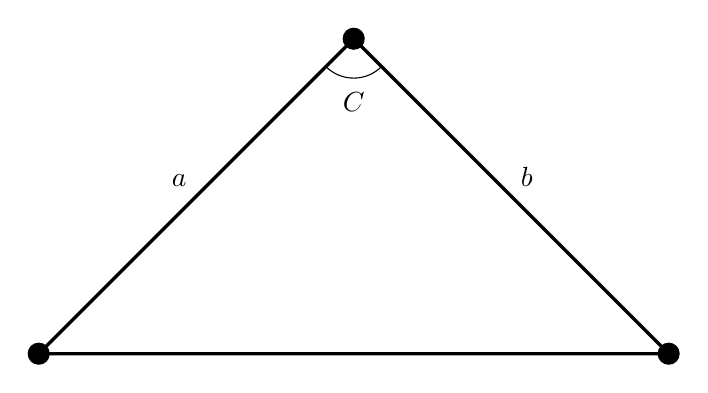
\begin{tikzpicture}[scale=2]
  % Define vertices
  \coordinate (A) at (0,0);
  \coordinate (B) at (4,0);
  \coordinate (C) at (2,2);

  % Draw triangle
  \draw[very thick] (A) -- (B) -- (C) -- cycle;

  % Draw dots at vertices
  \fill (A) circle (2pt);
  \fill (B) circle (2pt);
  \fill (C) circle (2pt);

  % Draw angle arc at C
  \draw pic["$C$", draw, angle radius=0.5cm, angle eccentricity=1.6] {angle=A--C--B};

  % Label sides
  \node[above left] at ($(A)!0.5!(C)$) {$a$};
  \node[above right] at ($(B)!0.5!(C)$) {$b$};
\end{tikzpicture}
\end{document}
